\section{Strategic Reasoning}

Antonio Gramsci, in his \textit{Prison Notebooks}, made a breakthrough in understanding revolution by disaggregating the Marxian concept of class warfare into two parts: the ``war of maneuver'' and the ``war of position''. The ``war of maneuver'' is the type of thing we imagine when we think of the word ``war'': direct, violent confrontation with the oppressors/exploiters. When the rebels in the Sierra Maestra slowly made their way through Cuba engaging in armed battles against Batista's forces, they were carrying out a ``war of maneuver''. However, as Gramsci argued, a group can't simply get together one day and decide to go ahead and directly confront the exploiters. In any act of revolution, they also need to work to gain a following among the exploited, establishing ``footholds'' among various sectors of society so they have a strong ``position'' in said society from which to attack (hence the name).

In the Russian Revolution, for example, years of organizing and agitation among workers -- who formed the vast majority of the Russian army (just like the US army today) -- ensured that when Kerensky ordered troops to fire upon the Bolsheviks storming the Winter Palace, they refused and abandoned their posts \textit{en masse}. One can see the salience and importance of Gramsci's idea here by imagining what would have happened if the Bolsheviks had ignored the war of position and solely focused on the war of maneuver -- for example, if they had spent all their time doing military drills and studying battlefield maps instead of going across the country organizing future soldiers in their workplaces.

In fact, we don't even have to go back to the 20th century for an example of the crucial role played by the war of position. The 2003 film \textit{The Revolution Will Not Be Televised} documents the attempted US coup against Hugo Chavez in Venezuela, with the camera crew capturing the pivotal moment in the coup's failure when a member of the palace guard suddenly looks over to the camera and holds up a fist. With this gesture, the guard signaled to the millions of protesters outside that that they had not abandoned Chavez and presaged the storming of the Palace by the guards shortly thereafter, driving the US-backed forces out and sounding the death knell for the US's plan.

Thus, at the end of this section, we'll encounter the strategic situation that should be at the front of any anti-capitalist's mind: the ``Revolution Game''. Before we get there, however, we'll need to know the basics. Long story short, unless you end up doing game theory as a profession, you just need to know two standard formats for representing strategic situations: games in ``Normal Form'' and games in ``Extensive Form''.

\subsection{Normal Form Games: Rock, Paper, Scissors}

Normal Form games are the simpler case: essentially they allow us to represent strategic situations where there is a \textit{single} decision that needs to be made, by two or more agents\footnote{Although, above 3 agents the diagrams you'll need to make start looking kinda gross.} who act \textit{simultaneously}. Think Rock, Paper, Scissors: if you were allowed to wait until the other player made a move to choose your own move, the game would be pretty dumb. In fact, let's look at Rock, Paper, Scissors in Normal Form for our first example (I'll explain everything in a minute):

\begin{table}[ht!]
    \centering
    \setlength{\extrarowheight}{2pt}
    \begin{tabular}{cc|c|c|c|}
      & \multicolumn{1}{c}{} & \multicolumn{3}{c}{Column Player ($C$)}\\
      & \multicolumn{1}{c}{} & \multicolumn{1}{c}{\strat{Rock}}  & \multicolumn{1}{c}{\strat{Paper}} & \multicolumn{1}{c}{\strat{Scissors}} \\\cline{3-5}
      \multirow{3}*{Row Player ($R$)}  & \strat{Rock} & $(0,0)$ & $(-1,1)$ & $(1,-1)$ \\\cline{3-5}
      & \strat{Paper} & $(1,-1)$ & $(0,0)$ & $(-1,1)$ \\\cline{3-5}
      & \strat{Scissors} & $(-1,1)$ & $(1,-1)$ & $(0,0)$ \\\cline{3-5}
    \end{tabular}
\label{fig:rps2}
\caption{Two-Player Simultaneous Rock, Paper, Scissors game in Normal Form}
\end{table}

The way to read this is, first off, to notice that each row in the matrix (the boxed numbers part) corresponds to one of the moves that the Row Player $R$ can make, while each column corresponds to a move that the Column Player $C$ can make. Thus, the full rules of the game are all there in the cells. To see what happens when Row Player plays Paper while Column Player plays Scissors, for example, we just look at the cell in the Paper ($P$) row and Scissors ($S$) column (2nd row, 3rd column). The two numbers represent the number of points each player gets in this situation, where the first number is how many points Row Player gets and the second is how many points Column Player gets. In our example, since Paper gets cut by Scissors, Row Player loses and gets $-1$ points while Column Player wins and receives $1$ point. If both played Rock instead, the cell at row Rock ($K$) and column Rock ($K$) (1st row, 1st column) tells us that the players both get no points.

We'll learn what we can actually \textit{do} with these matrices soon enough. First, though, note that we can easily extend this format to 3 players: instead of one table we can construct three, and then which of the three we look at is determined by the strategy chosen by Third Player ($T$). Let's make a 3-player version of Rock, Paper, Scissors where you get points based on how you match against two other people. For example, if Third Player plays \strat{Scissors} and the two other players play \textsf{Paper}, Third Player gets two points. But if Third Player plays \textsf{Scissors} while Row Player plays \textsf{Paper} and Column Player plays \textsf{Rock}, then Third Player gets one point for beating Row Player but \textit{loses} one point as well for losing to Column Player. This looks like the following:

\begin{table}
\centering
    \setlength{\extrarowheight}{2pt}
    \textbf{\underline{(a) Third Player ($T$) chooses \strat{Rock}}}:
    \begin{tabular}{cc|c|c|c|}
      & \multicolumn{1}{c}{} & \multicolumn{3}{c}{Column Player ($C$)}\\
      & \multicolumn{1}{c}{} & \multicolumn{1}{c}{\strat{Rock}}  & \multicolumn{1}{c}{\strat{Paper}} & \multicolumn{1}{c}{\strat{Scissors}} \\\cline{3-5}
      \multirow{3}*{Row Player ($R$)}  & \strat{Rock} & RRR $(0,0,0)$ & RPR $(-1,2,-1)$ & RSR $(1,-2,1)$ \\\cline{3-5}
      & \strat{Paper} & PRR $(-2,1,1)$ & PPR $(1,1,-2)$ & PSR $(0,0,0)$ \\\cline{3-5}
      & \strat{Scissors} & SRR $(-2,1,1)$ & SPR $(0,0,0)$ & SSR $(-1,-1,2)$ \\\cline{3-5}
    \end{tabular}
    
    ~\\\rule{0pt}{4ex}
    
    \textbf{\underline{(b) Third Player ($T$) chooses \strat{Paper}}}:
    \begin{tabular}{cc|c|c|c|}
      & \multicolumn{1}{c}{} & \multicolumn{3}{c}{Column Player ($C$)}\\
      & \multicolumn{1}{c}{} & \multicolumn{1}{c}{\strat{Rock}}  & \multicolumn{1}{c}{\strat{Paper}} & \multicolumn{1}{c}{\strat{Scissors}} \\\cline{3-5}
      \multirow{3}*{Row Player ($R$)}  & \strat{Rock} & RRP $(-1,-1,2)$ & RPP $(-2,1,1)$ & RSP $(0,0,0)$ \\\cline{3-5}
      & \strat{Paper} & PRP $(1,-2,1)$ & PPP $(0,0,0)$ & PSP $(-1,2,-1)$ \\\cline{3-5}
      & \strat{Scissors} & SRP $(0,0,0)$ & SPP $(2,-1,-1)$ & SSP $(1,1,-2)$ \\\cline{3-5}
    \end{tabular}
    
    ~\\\rule{0pt}{4ex}
    
    \textbf{\underline{(c) Third Player ($T$) chooses \strat{Scissors}}}:
    \begin{tabular}{cc|c|c|c|}
      & \multicolumn{1}{c}{} & \multicolumn{3}{c}{Column Player ($C$)}\\
      & \multicolumn{1}{c}{} & \multicolumn{1}{c}{\strat{Rock}}  & \multicolumn{1}{c}{\strat{Paper}} & \multicolumn{1}{c}{\strat{Scissors}} \\\cline{3-5}
      \multirow{3}*{Row Player ($R$)} & \strat{Rock} & RRS $(1,1,-2)$ & RPS $(0,0,0)$ & RSS $(2,-1,-1)$ \\\cline{3-5}
      & \strat{Paper} & PRS $(0,0,0)$ & PPS $(-1,-1,2)$ & PSS $(-2,1,1)$ \\\cline{3-5}
      & \strat{Scissors} & SRS $(-1,2,-1)$ & SPS $(1,-2,1)$ & SSS $(0,0,0)$ \\\cline{3-5}
    \end{tabular}
\label{fig:rps3}
\caption{Three-Player Simultaneous Rock, Paper, Scissors in Normal Form}
\end{table}

As before, the numbers represent the payoffs for the players in each possible outcome. You first use Third Player's chosen action to pick a table, then you find the correct row and column just as before (3rd row, 3rd column). The only difference is the additional 3rd number in the cells now, which represents the payoff for Third Player (with the first two being, as before, Row Player points and Column Player points, in that order). For example, if Row Player plays \strat{Paper}, Column Player chooses \strat{Rock}, and Third Player chooses \strat{Paper}, we look in the 2nd row, 1st column of the 2nd table. We see the payoff profile $(1,-2,1)$, which indicates that Row Player receives 1 point (they beat Column Player's \strat{Rock} with their \strat{Paper} and tied Third Player), Column Player loses 2 points (their \strat{Rock} loses to both the \strat{Paper} chosen by Row Player \textit{and} the \strat{Paper} chosen by Third Player), and Third player receives 1 point (for tying Row Player and beating Column Player's \strat{Rock} with their \strat{Paper}).

If you think about it geometrically, this is equivalent to a $3 \times 3 \times 3$ cube of possible outcomes rather than a $3 \times 3$ square like we had above. Hence since we can imagine 3D cubes, but have a harder time visualizing hypercubes\footnote{Visualizing a 4D hypercube is not too bad if you just imagine a 3D cube with a ``time slider'' underneath it, such that the entries in the cube change as you drag the slider (the cube is ``moving through'' the time dimension). But above that I've got nothing.}, I don't recommend trying to model strategic situations with more than 3 agents this way.

But let's explore another way of representing these types of situations: the Extensive Form. Here I get to use my favorite example, which (I'm sorry) comes from sports: the \href{https://en.wikipedia.org/wiki/Barbados_4\%E2\%80\%932_Grenada_(1994_Caribbean_Cup_qualification)}{1994 Caribbean Cup qualification match} between Barbados and Grenada. The rules in this match were basically the same as standard international-competition rules, with one twist: if the game goes into overtime and a team scores a ``golden goal'' (a goal scored in overtime is ``golden'' in that the game immediately ends and the team who scored wins), they are given \textit{two} points instead of one. As in, if the game was tied 10--10 going into overtime, and the first team scored a goal, the final score would be 12--10. Chaos ensued, however, when Barbados noticed that they were winning 2--1 with only 3 minutes left. It turned out, due to math, that they actually needed to win by \textit{two} points or more in order to advance to the tournament\footnote{The qualifying round of a soccer tournament involves assigning each team to a mini-``league'', where each league has 4 teams total. Every team then plays each other team one time, and after all the games are finished the teams within each league are sorted based on their number of wins, where ties in number of wins are broken based on \textit{goal differential} -- the number of goals a team scored minus the number of goals that were scored on them. This produces the unambiguous final standings of who will enter the subsequent single-elimination tournament and who will not advance.}, because when there are ties with respect to number of wins the teams' goal differentials (number of goals scored minus number of goals given up) are used as the tiebreaker. Noticing this in a galaxy brain moment, Barbados quickly ran over to their own goal and purposefully scored an own-goal. Why? It's time for some game theory folks $\ldots$ Let's map this situation out using the new Extensive Form, which I'll explain in a moment:

~\\

%\begin{tikzpicture}[scale=1.5,font=\footnotesize]
%% Specify spacing for each level of the tree
%\tikzstyle{level 1}=[level distance=15mm,sibling distance=35mm]
%\tikzstyle{level 2}=[level distance=15mm,sibling distance=15mm]
%% The Tree
%\node(0)[solid node,label=above:{Barbados}]{}
%child{node(1)[solid node]{}
%child{node[hollow node,label=below:{$(a,b)$}]{} edge from parent node[left]{$C$}}
%child{node[hollow node,label=below:{$(c,d)$}]{} edge from parent node[right]{$D$}}
%edge from parent node[left,xshift=-3]{$A$}
%}
%child{node(2)[solid node]{}
%child{node[hollow node,label=below:{$(e,f)$}]{} edge from parent node[left]{$C$}}
%child{node[hollow node,label=below:{$(g,h)$}]{} edge from parent node[right]{$D$}}
%edge from parent node[right,xshift=3]{$B$}
%};
%\end{tikzpicture}

\begin{figure}
\centering
\begin{tikzpicture}[scale=1,font=\footnotesize,edge from parent/.style={line width=1,draw}]
% Two node styles: solid and hollow
\tikzstyle{solid node}=[circle,draw,inner sep=1.2,fill=black];
\tikzstyle{hollow node}=[circle,draw,inner sep=1.2];
% Specify spacing for each level of the tree
\tikzstyle{level 1}=[level distance=30mm,sibling distance=50mm]
\tikzstyle{level 2}=[level distance=30mm,sibling distance=25mm]
% The Tree
\node(0)[hollow node]{}
child{node{}
edge from parent
node[line width=1,inner sep=3.5,fill=white,draw=black]{\strat{Rock}}
}
child{node{}
edge from parent
node[line width=1,inner sep=3.5,fill=white,draw=black]{\strat{Paper}}
}
child{node{}
edge from parent
node[line width=1,inner sep=3.5,fill=white,draw=black]{\strat{Scissors}}
};
\draw[dashed,rounded corners=7]($(0-1)+(-.3,0.15)$)rectangle($(0-3)+(.3,-0.38)$);
% movers
\node[above,circle,inner sep=1,yshift=-20]at(0){Third Player};
\node[below,yshift=-7]at(0-1){
\arrayrulewidth0.75pt
\setlength{\tabcolsep}{1.6pt}
\small{
\begin{tabular}{|c|c|c|}\hline
$0,0,0$ & $-1,2,-1$ & $1,-2,1$\\\hline
$-2,1,1$ & $1,1,-2$ & $0,0,0$\\\hline
$-2,1,1$ & $0,0,0$ & $-1,-1,2$ \\\hline
\end{tabular}}
};
\node[below,yshift=-7,xshift=-2]at(0-2){
\arrayrulewidth.75pt
\setlength{\tabcolsep}{1.5pt}
\small{
\begin{tabular}{|c|c|c|}\hline
$-1,-1,2$ & $-2,1,1$ & $0,0,0$ \\\hline
$1,-2,1$ & $0,0,0$ & $-1,2,-1$ \\\hline
$0,0,0$ & $2,-1,-1$ & $1,1,-2$ \\\hline
\end{tabular}}
};
\node[below,yshift=-7]at(0-3){
\arrayrulewidth.75pt
\setlength{\tabcolsep}{1.5pt}
\small{
\begin{tabular}{|c|c|c|}\hline
$1,1,-2$ & $0,0,0$ & $2,-1,-1$\\\hline
$0,0,0$ & $-1,-1,2$ & $-2,1,1$\\\hline
$-1,2,-1$ & $1,-2,1$ & $0,0,0$\\\hline
\end{tabular}}
};
%\node [circle, draw=black,yshift=-4] at (0-1) {};
\node[yshift=-5] at ($.333*(0-1)+.333*(0-2)+.333*(0-3)$) {Row Player, Column Player};
\end{tikzpicture}
\caption{Simultaneous Rock, Paper, Scissors in Extensive Form\label{fig:simrps}}
\end{figure}

\begin{figure}
\centering
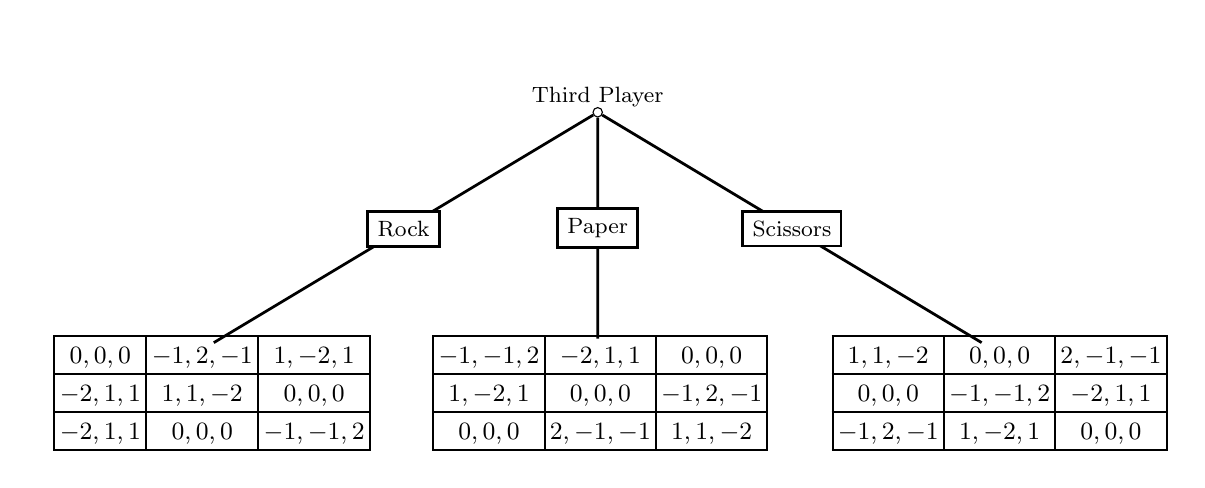
\begin{tikzpicture}[scale=1,font=\footnotesize,edge from parent/.style={line width=1,draw}]
% Two node styles: solid and hollow
\tikzstyle{solid node}=[circle,draw,inner sep=1.2,fill=black];
\tikzstyle{hollow node}=[circle,draw,inner sep=1.2];
% Specify spacing for each level of the tree
\tikzstyle{level 1}=[level distance=30mm,sibling distance=50mm]
\tikzstyle{level 2}=[level distance=30mm,sibling distance=25mm]
% The Tree
\node(0)[hollow node]{}
child{node{}
edge from parent
node[line width=1,inner sep=3.5,fill=white,draw=black]{\strat{Rock}}
}
child{node{}
edge from parent
node[line width=1,inner sep=3.5,fill=white,draw=black]{\strat{Paper}}
}
child{node{}
edge from parent
node[line width=1,inner sep=3.5,fill=white,draw=black]{\strat{Scissors}}
};
% movers
\node[above,circle,inner sep=1,yshift=-20]at(0){Third Player};
\node[below,yshift=8.5]at(0-1){
\arrayrulewidth0.75pt
\setlength{\tabcolsep}{1.6pt}
\small{
\begin{tabular}{|c|c|c|}\hline
$0,0,0$ & $-1,2,-1$ & $1,-2,1$\\\hline
$-2,1,1$ & $1,1,-2$ & $0,0,0$\\\hline
$-2,1,1$ & $0,0,0$ & $-1,-1,2$ \\\hline
\end{tabular}}
};
\node[below,yshift=8.5,xshift=-2]at(0-2){
\arrayrulewidth.75pt
\setlength{\tabcolsep}{1.5pt}
\small{
\begin{tabular}{|c|c|c|}\hline
$-1,-1,2$ & $-2,1,1$ & $0,0,0$ \\\hline
$1,-2,1$ & $0,0,0$ & $-1,2,-1$ \\\hline
$0,0,0$ & $2,-1,-1$ & $1,1,-2$ \\\hline
\end{tabular}}
};
\node[below,yshift=8.5]at(0-3){
\arrayrulewidth.75pt
\setlength{\tabcolsep}{1.5pt}
\small{
\begin{tabular}{|c|c|c|}\hline
$1,1,-2$ & $0,0,0$ & $2,-1,-1$\\\hline
$0,0,0$ & $-1,-1,2$ & $-2,1,1$\\\hline
$-1,2,-1$ & $1,-2,1$ & $0,0,0$\\\hline
\end{tabular}}
};
\end{tikzpicture}
\caption{Sequential Rock, Paper, Scissors in Extensive Form\label{fig:seqrps}}
\end{figure}

%%%%%
%%% Barbados game
%%%%%

\begin{figure}
\centering
\begin{tikzpicture}[scale=1,font=\footnotesize,edge from parent/.style={line width=1,draw}]
% Two node styles: solid and hollow
\tikzstyle{solid node}=[circle,draw,inner sep=1.2,fill=black];
\tikzstyle{hollow node}=[circle,draw,inner sep=1.2];
% Specify spacing for each level of the tree
\tikzstyle{level 1}=[level distance=30mm,sibling distance=50mm]
\tikzstyle{level 2}=[level distance=30mm,sibling distance=25mm]
% The Tree
\node(0)[hollow node]{}
child{node{}
edge from parent
node[line width=1,inner sep=3.5,fill=white,draw=black]{\strat{Do Nothing}}
}
child{node{}
edge from parent
node[line width=1,inner sep=3.5,fill=white,draw=black]{\strat{Own Goal}}
};
% movers
\node[above,circle,inner sep=1,yshift=-10]at(0){Barbados};
\node[below,yshift=-7]at(0-1){
\arrayrulewidth0.75pt
\setlength{\tabcolsep}{1.6pt}
test1
};
\node[below,yshift=-7,xshift=-2]at(0-2){
\arrayrulewidth.75pt
\setlength{\tabcolsep}{1.5pt}
test2
};
%\node [circle, draw=black,yshift=-4] at (0-1) {};
\node[yshift=-5] at ($.333*(0-1)+.333*(0-2)+.333*(0-3)$) {Row Player, Column Player};
\end{tikzpicture}
\caption{Double Golden Goal Game (Extensive Form)\label{fig:dgg}}
\end{figure}

\subsection{The Revolution Game}

In this game from \cite{mccarty_political_game_theory}, an imperialist country $B$ rules over a colony $A$, and in each ``round'' (here we'll assume a ``round'' spans over the course of 1 year) $A$ and $B$ interact via the following sequential steps (i.e., steps performed in order, such that the actions taken in previous steps are observed/known by whoever is currently making a decision)\footnote{The game ends up pretty much perfectly, though [almost surely] inadvertently, illustrating Gramsci's strategic dichotomy. I've changed the descriptions only a tiny bit here, to match up with the context of the chapter, since (e.g.) the book does not ever cite or mention Gramsci.}:
\begin{enumerate}
    \item A revolutionary group in the colony (which we'll metonymically just also call $A$, for better or worse) decides whether to Revolt and storm the palace ($R$) this year, or to Continue agitating among the population ($C$) during the year, and then
    \item Officials in the metropole (who we similarly refer to as $B$) decide upon a response as follows (based on $A$'s choice):
    \begin{enumerate}
        \item If $A$ chose to Revolt, they decide between caving in and Granting independence ($G$) or violently Suppressing the revolt ($S$).
        \item If $A$ chose to Continue agitating, they decide whether to continue Taxing the colonial population ($T$) or to Eliminate taxes as a preventative measure to lower the (immediate) likelihood of revolt.
    \end{enumerate}
\end{enumerate}
The interesting thing about this game, however, compared to the Rock, Paper, Scissors games we looked at above, is that the sequential rather than simultaneous nature of the choices here requires that the imperial metropole $B$ come up with a policy specifying what to do in \textit{both} of the cases they might end up in: a ``strategy'' for this game, in $B$'s case, is not just a single action choice or even a probability distribution over action choices (like we saw in the Rock, Paper, Scissors cases) but rather a \textit{conditional} policy stating ``if $A$ chooses Revolt, do $X$, otherwise do $Y$''. Any valid strategy for $B$ in this game takes on this form, with $X$ and $Y$ filled in with particular choices. We can represent these strategies in mathematical shorthand as $\{R \rightarrow X, C \rightarrow Y\}$, so that for example the strategy ``If $A$ chooses Revolt, choose Suppress, otherwise choose continue Taxing'' can be shortened to
\begin{align*}
    \{R \rightarrow S, C \rightarrow T\}.
\end{align*}
Finally, before we can start analyzing the game, we need to specify the payoff profile, i.e., how much utility each agent would receive in every possible outcome.

To start with, the key stakes of the colonial extraction here revolve around control of a lucrative oil field in the colony $B$, which generates 4 utils per year for whoever controls it.

Organizing and carrying out a Revolt costs $A$ one util \textit{if} it is not met with Suppression, but if it is then the Revolt costs $A$ 6 utils, and the Suppression itself costs $B$ 6 utils. In the latter case, the relative strengths of the two armies gives rise to some probability $p$ that the Revolt succeeds, in the sense that $A$ is able to gain control over its oil field (and thus the revenue deriving from it) during the round and no longer has to pay taxes to $B$, with a corresponding probability of $1-p$ that the Revolt fails and $B$ retains control over the oil field and continues to collect taxes from $A$.

In the case where $A$ chooses not to Revolt, $B$ receives 2 utils via taxation (meaning that, at the end of the round, $B$ gains 2 utils while $A$ loses 2 utils) if they decide to Continue taxing $A$, or 0 utils via taxation if they decide to Eliminate the tax. So in total we have four possible outcomes, with the payoff profile as follows:
\begin{itemize}
    \item \textbf{[Outcome $O_1 = (R,G)$] $A$ chooses Revolt, $B$ chooses to Grant independence}: $A$ receives a payoff of $\pi_A(O_1) = 3$ utils (4 utils via oil field revenue minus the 1 util ``spent'' on organizing and carrying out the Revolt) and $B$ receives a payoff of $\pi_B(O_1) = 0$ utils, so that the payoff tuple for this outcome is $\pi(O_1) = (\pi_A(O_1),\pi_B(O_1)) = (3,0)$.
    \item \textbf{[Outcome $O_2 = (R,S)$] $A$ chooses Revolt, $B$ chooses to Suppress the revolt}: Here, as described above, the Revolt succeeds with probability $p$ and fails with probability $1-p$, so that
    \begin{itemize}
        \item In the case where the Revolt succeeds, $A$ successfully derives 4 utils from the newly-controlled oil field revenues, and no longer has to pay a tax to $B$, but still loses 6 utils due to the damage from the Suppression, for a net payoff of $4-6 = -2$ utils. $B$, on the other hand, loses 6 utils ``paying for'' the Suppression and no longer gains any utils from taxation or from the oil fields, resulting in a net payoff of $0-6 = -6$ utils.
        \item In the case where the Revolt fails, $A$ loses 6 utils due to the damage from the Suppression, plus they must continue paying taxes to $A$ and thus lose an additional 2 utils, for a net payoff of $0-8 = -8$ utils. $B$ also loses 6 utils carrying out the Suppression, but gains their usual 4 utils from the oil field revenues and 2 utils from taxation of $B$, for a net payoff of $6-6 = 0$ utils.
    \end{itemize}
    Although we can't derive \textit{numeric} values for the payoff tuple $\pi(O_2) = (\pi_A(O_2), \pi_B(O_2))$ here without knowing the numeric value of $p$, we can leave $p$ as an unknown variable and still derive a useful expression for the payoff tuple by writing these payoffs as a \textit{function} of $p$. To do so we ``re-cast'' the payoff tuple $\pi(O)$, for some outcome $O$, as representing the \textit{expected} amount of utility $A$ and $B$ will receive from outcome $O$\footnote{This ``re-casting'' doesn't affect the deterministic payoff values we've already seen, like those of the previous case $O_1$, since the expected value of a non-random quantity is just the quantity itself, by definition. So for the previous outcome $O_1$, with our new definition of $\pi$, we still have
    \begin{align*}
        \pi(O_1) = (\pi_A(O_1),\pi_B(O_1)) = (E[U_A(O_1)], E[U_B(O_1)]) = (E[3],E[0]) = (3,0).
    \end{align*}}. Then we can compute the payoff tuple values as follows, where we also define a helpful ``indicator variable'' $W$ that just numerically represents whether or not the Revolt was successful by taking on the value 1 if it was and 0 otherwise:
    \begin{align*}
        % expected utility for A
        \pi_A(O_2) = E[U_A(O_2)] &= E[U_A((R,S))] = E[U_A(O_2)\given{}W=1] + E[U_A(O_2)\given{}W=0] \\
        &= P(W=1)\cdot U_A(O_2\given{}W=1) + P(W=0)\cdot U_A(O_2\given{}W=0) \\
        &= p\cdot U_A(O_2\given{} W=1) + (1-p)\cdot U_A(O_2\given{} W=0) \\
        &= p\cdot(-2) + (1-p)\cdot(-8) = -2p - 8 + 8p = 6p - 8, \\
        % expected utility for B
        \pi_B(O_2) = E[U_B(O_2)] &= E[U_B((R,S))] = E[U_B(O_2)\given{}W=1] + E[U_B(O_2)\given{}W=0] \\
        &= P(W=1)\cdot U_B(O_2\given{}W=1) + P(W=0)\cdot U_B(O_2\given{}W=0) \\
        &= p\cdot U_B(O_2\given{} W=1) + (1-p)\cdot U_B(O_2\given{} W=0) \\
        &= p\cdot(-6) + (1-p)\cdot(0) = -6p,
    \end{align*}
    so that now we can write the payoff tuple for this outcome as
    \begin{align*}
        \pi(O_2) = (\pi_A(O_2),\pi_B(O_2)) = (6p-8,-6p).
    \end{align*}
    \item \textbf{[Outcome $O_3 = (C,T)$] $A$ chooses to Continue organizing, $B$ chooses to continue Taxing $A$}: $A$ receives a payoff of $\pi_A(O_3) = -2$ utils (via the 2-util tax levied by $B$), and $B$ receives a payoff of $\pi_B(O_3) = 6$ utils (4 utils from the oil revenues plus 2 utils from the tax levied on $B$).
    \item \textbf{[Outcome $O_4 = (C,E)$] $A$ chooses to Continue organizing, $B$ chooses to Eliminate the tax}: $A$ receives a payoff of $\pi_A(O_4) = 0$ utils (since they no longer have to pay the 2-util tax), and $B$ receives a payoff of $\pi_B(O_4) = 4$ utils (via the revenue from the oil field).
\end{itemize}
With the payoff tuples now defined and computed for every possible outcome, we can create the Extensive Form representation of the game, as illustrated in Figure \ref{fig:revgame-ext}.


\begin{figure}
\centering
\begin{tikzpicture}[scale=1,font=\footnotesize,edge from parent/.style={line width=1,draw}]
% Two node styles: solid and hollow
\tikzstyle{solid node}=[circle,draw,inner sep=1.2,fill=black];
\tikzstyle{hollow node}=[circle,draw,inner sep=1.2];
% Specify spacing for each level of the tree
\tikzstyle{level 1}=[level distance=30mm,sibling distance=75mm]
\tikzstyle{level 2}=[level distance=30mm,sibling distance=25mm]
% The Tree
\node(0)[hollow node]{}
child{node{}
edge from parent
node[line width=1,inner sep=3.5,fill=white,draw=black]{\strat{Revolt ($R$)}}
}
child{node{}
edge from parent
node[line width=1,inner sep=3.5,fill=white,draw=black]{\strat{Continue Organizing ($C$)}}
};
% movers
\node[above,circle,inner sep=1,yshift=-10]at(0){Revolutionary Movement $A$};
\node[below,yshift=-7]at(0-1){
\arrayrulewidth0.75pt
\setlength{\tabcolsep}{1.6pt}
}
child{node{}}
child{node{}};
\node[below,yshift=-7,xshift=-2]at(0-2){
\arrayrulewidth.75pt
\setlength{\tabcolsep}{1.5pt}
test2
};
%\node [circle, draw=black,yshift=-4] at (0-1) {};
\end{tikzpicture}
\caption{Double Golden Goal Game (Extensive Form)\label{fig:dgg}}
\end{figure}

So, for this game, the structure of the Extensive Form representation actually helps us visualize the ``flow'' of the game, with the vertical ``axis'' representing the passage of time as we move from top to bottom -- unlike in World Cup or Rock, Paper, Scissors games where, frankly, we only looked at their Extensive Form representations so we could start getting comfortable with the idea that games always have more than one possible mode of representation. To drive this point home, though, let's see how we would represent this game in Normal form.

First, 

The game is represented in strategic normal form in Figure \ref{fig:revgame}.

\begin{table}[ht!]
    \centering
    \setlength{\extrarowheight}{2pt}
    \begin{tabular}{cc|c|c|}
      & \multicolumn{1}{c}{} & \multicolumn{2}{c}{Palace Guards ($G$)}\\
      & \multicolumn{1}{c}{} & \multicolumn{1}{c}{Fire ($F$)}  & \multicolumn{1}{c}{Stand Down ($SD$)} \\\cline{3-4}
      \multirow{2}*{Revolutionary Army ($R$)}  & Storm ($S$) & $(-100,100)$ & $(100,90)$ \\\cline{3-4}
      & Organize ($O$) & $(0,0)$ & $(0,0)$ \\\cline{3-4}
    \end{tabular}
\label{fig:revgame}
\end{table}

\subsection{Rules Without Rulers: The Stoplight Game}

% https://codesachin.wordpress.com/2015/11/11/traffic-lights-and-nash-equilibrium/

I grew up in a (purportedly) ``libertarian'' family, which in America really just means ``we don't like anything the government does, but we like anything a private corporation does''. I was raised to pass a stoplight and immediately think ``arbitrary big government imposition on our lives''! So this particular game blew my mind, and made me wonder (to this very day) what other institutions could be mathematically-justified as improving the welfare of all participants?

Picture yourself in an alternate Hobbesian world in which stoplights have been abolished, and imagine two cars both arriving at an intersection at the same time. By now you know the drill -- we'll model the situation as follows: (1) if both cars go, they crash and both drivers receive -10 utils, (2) if neither car goes, they sit there forever and receive -3 utils from the boredom, and (3) if one car goes but the other doesn't, the car that goes receives $4$ utils for safely getting to their destination, and the other car receives $-1$ utils for having to wait for the other car to go before they could go:
\begin{table}[ht!]
    \centering
    \setlength{\extrarowheight}{2pt}
    \begin{tabular}{cc|c|c|}
      & \multicolumn{1}{c}{} & \multicolumn{2}{c}{Car $B$}\\
      & \multicolumn{1}{c}{} & \multicolumn{1}{c}{Go ($G$)}  & \multicolumn{1}{c}{Don't Go ($D$)} \\\cline{3-4}
      \multirow{2}*{Car $A$}  & Go ($G$) & $(-10,-10)$ & $(4,-1)$ \\\cline{3-4}
      & Don't Go ($D$) & $(-1,4)$ & $(-3,-3)$ \\\cline{3-4}
    \end{tabular}
\label{fig:stoplight}
\end{table}

So what are the Nash equilibria here? (1) If Car $A$ decides to go, Car $B$'s best response is to not go (and receive $-1$ utils). (2) If Car $A$ decides not to go, Car $B$'s best response is to go (and receive 4 utils). The same logic holds for Car $A$ analyzing Car $B$'s potential moves, resulting in a table that looks like:
\begin{table}[ht!]
    \centering
    \setlength{\extrarowheight}{2pt}
    \begin{tabular}{cc|c|c|}
      & \multicolumn{1}{c}{} & \multicolumn{2}{c}{Car $B$}\\
      & \multicolumn{1}{c}{} & \multicolumn{1}{c}{Go ($G$)}  & \multicolumn{1}{c}{Don't Go ($D$)} \\\cline{3-4}
      \multirow{2}*{Car $A$}  & Go ($G$) & $(-10,-10)$ & $(\underline{\mathbf{4}},\underline{\mathbf{-1}})$ \\\cline{3-4}
      & Don't Go ($D$) & $(\underline{\mathbf{-1}},\underline{\mathbf{4}})$ & $(-3,-3)$ \\\cline{3-4}
    \end{tabular}
\label{fig:slnash}
\end{table}
